
Dieser Versuchsteil befasst sich mit der Messung der Momentanleistung an einem LCR-Schwingkreis, welcher unter Resonanzbedingung betrieben wird. Das Verhalten des Schwingkreises wird genauer untersucht und der Momentanleistungsverlauf wird erläutert.

\subsubsection{Versuchsaufbau}
Der Aufbau dieses Versuches ist identisch mit dem in Abschnitt \ref{sec:Aufbau2.2.1} verwendeten Aufbau. Einzig die Impedanzen werden verändert. Es gilt nun:
\begin{itemize}
\item $Z_1 = \frac{1}{j\omega C} \mbox{ mit } C=10\mu F $
\item $Z_2 = 40\Omega$
\item $Z_3 = R_{sp} + j\omega L \mbox{ mit } L=15,84mH$
\item $R_i$ wird nicht verändert. 
\end{itemize}

Das Oszilloskop wird weiterhin zur Messung der Momentanleistung über beliebige Verbraucher verwendet und wird wieder so eingestellt, dass die Momentanleistung als Produkt aus $u_I$ und $u_U$ angezeigt wird. Erneut gilt, dass die angezeigte Kurve nur proprotional zu $p(t)$ ist, da $R_i$ und somit $i(t)$, nicht exakt bekannt sind.

\subsubsection{Auswertung der Momentanleistungskurve}

Wie im in Abschnitt \ref{sec:Versuch2.2.1} erläuert wird die Momentanleistungskurve mit dem Oszilloskop aufgenommen. In Abbildung \ref{fig:MomLKurveResonanz} ist die zum Strom proportionale Kurve $u_I(t)$ in Blau, die Spannungskurve $u_U(t)$ in Rot und das zur Momentanleistung proportionale Produkt in grün.

\begin{figure}[H]
\centering
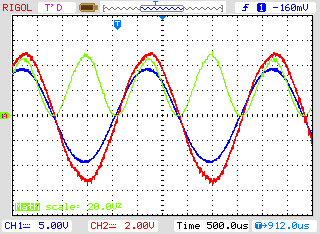
\includegraphics[width=0.7\linewidth]{Oszi-Bitmaps/NewFile4.jpg}
\caption{Momentanleistung eines LCR-Oszillators im Resonanzfall. $u_I(t)$ (Blau), $u_{Z_{ges}}(t)$ (Rot), $p_(t)$ (Grün)}
\label{fig:MomLKurveResonanz}
\end{figure}

Deutlich zu sehen ist die gleiche Phase von Strom und Spannung und die daraus resultierende, nur positive Momentanleistungskurve. Dies ist entgegen erster Intuition, da sich im Schaltkreis auch Verbraucher mit komplexer Impedanz befinden, welche normalerweise Blindleistung hinzufügen bzw. verbrauchen.
Begründen lässt sich dies jedoch, indem das Zeigerbild der über die einzelnen Verbraucher abfallende Spannung gezeichnet wird. Dieses ist in der Abbildung \ref{fig:ZeigerbildResonanz} zu sehen.

\begin{figure}[H]
\centering
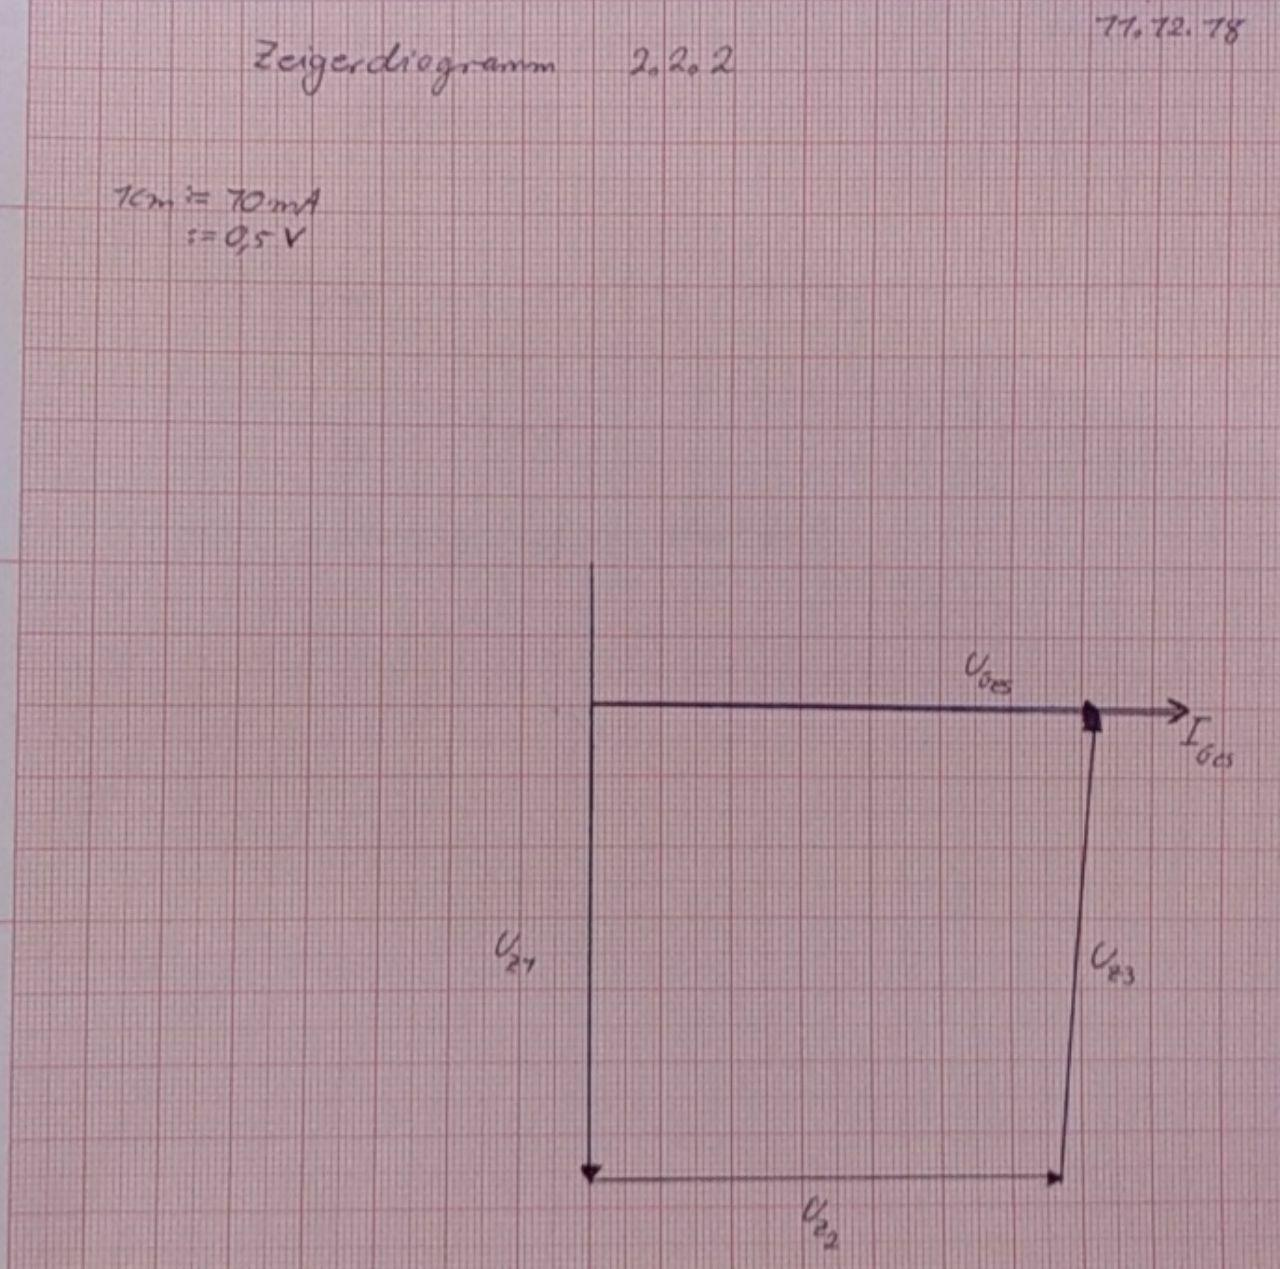
\includegraphics[width=0.7\linewidth]{Images/Zeigerdiagramm2-2-2.jpg}
\caption{Zeigerbild der Spannungen eines LCR-Schwingkreis im Resonanzfall}
\label{fig:ZeigerbildResonanz}
\end{figure}

Erkennbar ist die Phasenverschiebung von annähernd $180^\circ$ zwischen $\underline{U}_{Z1} \mbox{ und } \underline{U}_{Z2}$, welche lediglich durch den nicht vernachlässigbaren Innenwiderstand der Spule etwas kleiner ist. Auch ist zu sehen, dass $\underline{U}_{Z1} \mbox{ und } \underline{U}_{Z2}$ den gleichen Betrag besitzen. Die zwei Spannungen löschen sich fast komplett gegenseitig aus, das System verhält sich dementsprechend wie eine rein reelle Impedanz und besitzt keine Phasenverschiebung zwischen $\underline{U}_{ges}$ und $\underline{I}$. Dies ist typisches Verhalten für Schwingkreise im Resonanzfall und kann bei relativ geringen Innenwiderständen des Verbrauchers zu Schäden führen, sofern der Schaltkreis ungewollt anfängt zu schwingen.

Die komplexe Impedanz dieses Schaltkreises beträgt:
\begin{equation}
\underline{Z}_{ges} = \frac{1}{j\omega C} + R + R_{sp} + j\omega L = 45.5\Omega + j0.021\Omega
\end{equation}
Wie für einen resonierenden Schwingkreis erwartet verhält er sich von außen wie eine rein reelle Impedanz, der komplexe Teil ist vernachlässigbar klein. Somit nimmt er entsprechend Gleichung \eqref{eq:KomplexS} fast ausschließlich Wirkleistung auf.
